\section{Applying the C2W model}

\subsection{Language Modeling}
\label{subsec:language-model-c2w}

In this section we use the C2W model and a recurrent LSTM to perform language modeling as 
described in~\cite{DBLP:journals/corr/LingLMAADBT15}.
The neural network is going to compute the log propability $\log[ p(\mathcal{w}) ]$ of the 
sentence $\mathcal{w} = (w_1, \dots, w_m)$. As previously discussed in section~\ref{sec:language-modeling} this can be 
decomposed into the sum of the conditional log probabilities $log[ p(w_1,\dots,w_m) ] = \sum_{i=1}^{m} log[ p(w_i | w_1,\dots,w_{i-1}) ]$.
This model will compose the previously described word representations of $w_1,\dots,w_{i-1}$ to compute 
$log[ p(w_i | w_1,\dots,w_{i-1}) ]$ using a LSTM unit.
The model is shown in figure~\ref{fig:c2w-language-model}. The first stage can use either the embeddings generated with the C2W model
$f(w_i) = e_{w_i}^C $ or simply word lookup tables $e_{w_i}^W = P * 1_{w_i}$.

Every time we input a new word $w_i$ from the sequence we get the LSTM state $s_i$. The state $s_i$ is then used to predict word $w_{i+1}$.
The state $s_i$ is projected into a vector of size $|V|$ (the vocabulary size). The softmax is a $d \times V$ table, 
which encodes the likelihood of every word type in the vocabulary in a given context. 
The softmax layer will ensure a valid log probability distribution. This way we can choose the word type with the maximal likelihood.
Maximizing the conditional log-likelihoods during training will improve the modeling 
of $p(\mathcal{w})$~\cite{DBLP:conf/interspeech/MikolovKBCK10}.
More details regarding the softmax layer are explained in section~\ref{subsec:softmax}.

\begin{figure}[H]
\begin{center}
  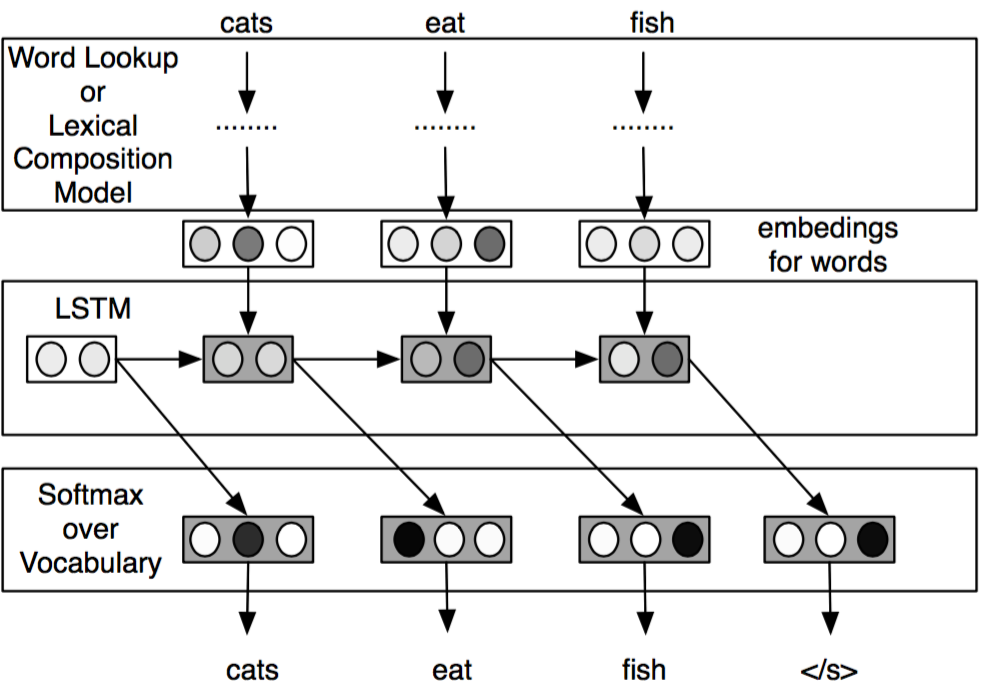
\includegraphics[width=0.6\textwidth]{./img/c2w-language-model}
  \caption{Neural network for language model. The C2W model is at the top, the word embeddings are then fed into an recurrent LSTM.}
  \label{fig:c2w-language-model}
\end{center}
\end{figure}


\subsubsection{Evaluation}

The original paper~\cite{DBLP:journals/corr/LingLMAADBT15} compares the performance of the language model 
in terms of it's perplexity~\ref{subsec:perplexity}. To minimize the perplexity value means to have a better fitting language model.
Perplexity cannot be used to compare models with different vocabularies,
since there are fewer outcomes in the softmax, the global perplexity can decrease.

In table~\ref{tab:perplexity} the perplexities and the parameter counts are displayed for different language models.
The language model performance is tested on English, Portuguese, Catalan, German and Turkish; the data is extracted from wikipedia.
Every word embedding $e_{w} \in \mathbb{R}^{d_w}$ is going to have $d_w = 50$ parameters.
Therefore the model using a lookup table of word embedding contains at least $d_w \cross |V|$ parameters.
The parameter count for the language model using C2W based embeddings depends on a few things. The number of parameters for each character
representation $d_C = 50$, and the number of parameters $d_{CS} = 150$ in the LSTM state $s_i$. The C2W model contains 8 matrices of 
size $d_{CS} \cross d_C + 2d_{CS}$ (One for each of the 4 decision gates in both LSTM's). Additionally there is the character lookup table 
which has an entry for every character in the language $d_C \cross |C|$. For English and 618 this works out to $15000 + 30900$ parameters.

\begin{table}
\begin{center}
\begin{tabular}{ l l l l l }
  \hline
             & \multicolumn{3}{|c|}{Fusional} &   \multicolumn{3}{|c|}{Agglutinative} \\ \hline
  Perplexity   & English & Portugese & Catalan & German & Turkish \\
  %5-gram KN    & 70.72   & 58.73     &   39.83 & 59.07  & 52.87   \\
  Word Lookup  & 59.38   & 46.17     &   35.34 & 43.02  & 44.01   \\
  C2W Model    & 57.39   & 40.92     &   34.92 & 41.94  & 32.88   \\
  #Parameters  &         &           &         &        &         \\
  Word Lookup  & 4.3M    & 4.2M      &  4.3M   & 6.3M   & 5.7M   \\
  C2W Model    & 180K    & 178K      &  182K   & 183K   & 174K   \\

\end{tabular}
\end{center}
\caption{Perplexities of different language models and the test configuration (From~\cite{DBLP:journals/corr/LingLMAADBT15}).}
\label{tab:perplexity}
\end{table}

% ==========================================================================================
\subsection{Part-of-Speech Tagging}

Part-of-Speech tagging is the process of labeling words as corresponding to a particular part of speech. A simple tagging would be
to identify words as nouns, verbs, adjectives, adverbs, etc.
The model receives a number of words $w_1,\dots,w_m$ as input, and transforms them into word embeddings. These embeddings are then processed
in a bidirectional LSTM layer, just as described in section~\ref{subsec:bidir-rnn}. 
In contrast to the combining layer of the C2W model, we don't just use the final state of the LSTM output states, but all states.
The forward states $s^f_0,\dots,s^f_m$ and the backward states  $s^n_m,\dots,s^b_0$ are combined with  $l_i = \tanh(L^f s_i^f + L^b s^b_i + b_l)$.
Where $L^f$, $L^b$, $b_l$ are the parameters of the combining layer. The output label for each word $w_i$ is then obtained from a softmax layer over
all word labels.

\begin{figure}[H]
\begin{center}
  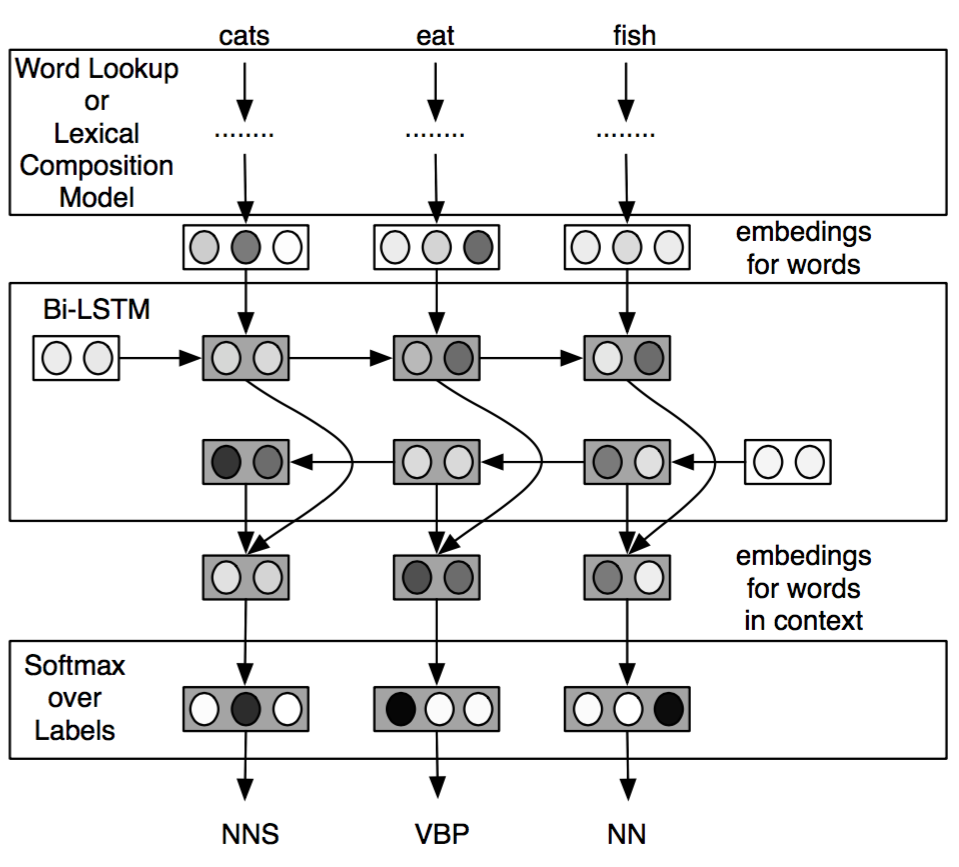
\includegraphics[width=0.6\textwidth]{./img/part-of-speech}
  \caption{The arhitecture of the NN for part-of-speech tagging (From~\cite{DBLP:journals/corr/LingLMAADBT15}).}
  \label{fig:c2w-language-model}
\end{center}
\end{figure}

\subsubsection{Evaluation}

The POS tagging is evaluated on the same languages as before. We compare the POS model with word embeddings from a lookup table
as well as Stanford’s POS tagger with the C2W based POS tagger.
\begin{table}
\begin{center}
\begin{tabular}{ l l l l l }
  \hline
  System       & \multicolumn{3}{|c|}{Fusional} &   \multicolumn{3}{|c|}{Agglutinative} \\ \hline
               & English & Portugese & Catalan & German & Turkish \\
  %5-gram KN    & 70.72   & 58.73     &   39.83 & 59.07  & 52.87   \\
  Word Lookup  & 96.97   & 95.67     &  98.09  & 97.51  & 83.43   \\
  C2W Model    & 97.36   & 97.47     &  98.92  & 98.08  & 91.59   \\
  Stanford     & 97.32   & 97.54     &  98.76  & 97.92  & 87.31  \\

\end{tabular}
\end{center}
\caption{Accuracy of the POS tagging in percent (From~\cite{DBLP:journals/corr/LingLMAADBT15}).}
\label{tab:pos-eval}
\end{table}


% ==========================================================================================
\subsection{Morphological inflection generation} 

Another application of C2W like model beyond language modeling is the morphological inflection generation~\cite{DBLP:journals/corr/FaruquiTND15}.
The goal is to perform a lingustic transformation some examples of the inflections which this model seeks to 
generate can be seen in table~\ref{tab:inflections}. First stage is the \textbf{encoder}:\\
This part of the model is eqvivalent to the C2W model: Each word $w$ is broken up into it's characters $e_{c_1}^C, \dots, e_{c_m}^C$.
Then a bidirectional LSTM layer is used and th result is composed into $e_{w}$.
Second part is the \textbf{decoder}:\\
This is a LSTM unit which will sequentially receive the word characters as input combined with the previous output and the word vector.
Every output state is computed as $s_t = g(s_{t-1}, \{e_{w}, y_{t-1}, x_t\})$. Where $g$ is the decoder LSTM unit,
$s_t$ is the LSTM output, $y_{t-1}$ the actual character output and $x_t$ is the current input character.
Since the input word might be shorter than the output, onece the input sequence runs out of characters we feed in an $\epsilon$ character
indicating null input: $x_t = \epsilon$. The vector representation for the $\epsilon$ character is learned just like in the C2W model.


\begin{figure}[H]
\begin{center}
  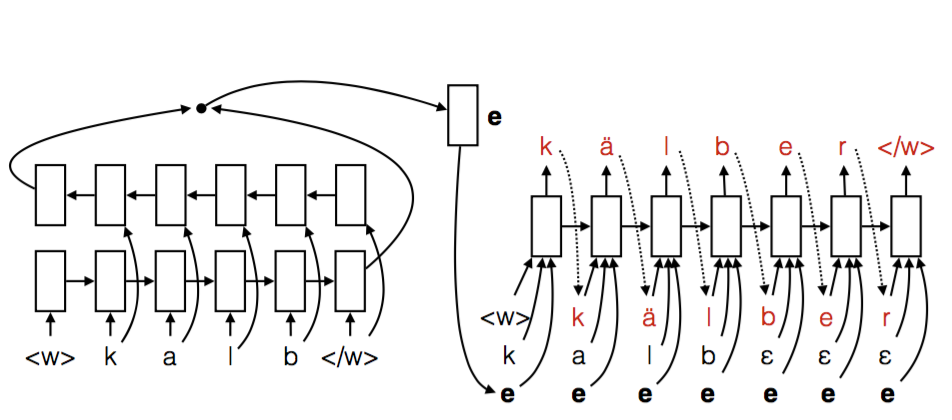
\includegraphics[width=\textwidth]{./img/inflection-generatior}
  \caption{A endoder decoder structure for inflection generation}
  \label{fig:inflection-generatior}
\end{center}
\end{figure}

\begin{table}
\begin{center}
\begin{tabular}{ l l l l }
  \hline
             & singular & plural \\ \hline
  nominative & Kalb & K\"alber \\
  accusative & Kalb & K\"alber \\
  dative & Kalb & K\"albern \\
  genitive & Kalbes & K\"alber \\
\end{tabular}
\end{center}
\caption{Example of an inflection table for the word Kalb (calf, German).}
\label{tab:inflections}
\end{table}

Converting the word embeddings from a C2W like model back into inflected versions of the word 
as discussed in Faruqui et al. \cite{DBLP:journals/corr/FaruquiTND15}

% Comparison of current LSTMs based word embeddings with the character based method from Santos et al. \cite{DBLP:conf/icml/2014}